\chapter{Experiments}
\label{chap:experiments}
To evaluate the research question we have conducted in total 11 experiments for every task.
We categorize experiments into 4 groups: Human performance, Baseline, Backbone models and Fine-tuning methods.

\section{Human performance}
\label{sec:human}
To evaluate human performance, we let 5 evaluators classify the articles on the Test-human set (see \autoref{enum:test-human}).

\section{Baseline}
For a baseline, we have used Multi-class Logistic Regression with TF-IDF features.
TF-IDF features setting was:
\begin{enumerate}
    \item Tokenization method: lowercased text with MosesTokenizer\footnote{https://pypi.org/project/mosestokenizer/}
    \item Maximum document frequency: 1\%
    \item Ngrams: 1-2
    \item Minimum document frequency: 90 documents
    \item Stop words: Czech stop words from stop-words package\footnote{https://pypi.org/project/stop-words/}
\end{enumerate}
Similar to \cite{strakaSumeCzechLargeCzech2018a} we have added the following additional features:
\begin{enumerate}
    \item Number of words
    \item Number of words with only non-alphabetic characters
    \item Number of uppercase words
    \item Number of digits words
    \item Number of capitalized words
\end{enumerate}


We run a grid search over the following hyperparameters:
\begin{enumerate}
    \item Inverse Regularization term: $1, 10, 100, 1000$
\end{enumerate}
We selected the best model based on the f1-macro score on the validation set.
As for the solver, we have used SAGA (\cite{defazioSAGAFastIncremental2014})
 implementation from Scikit-learn library\footnote{https://scikit-learn.org}.
with max iterations set to 800 and early stopping tolerance set to 0.001.
With this setting, we created 2 models; \textbf{LR-BASE-40} with 40k features
 and \textbf{LR-BASE-200} with 200k features.

\section{Backbone models}
\label{sec:backbone}
For backbone models, we have used \textbf{RobeCzech}, \textbf{Fernet-News}, and \textbf{GPT-3}.
We chose RobeCzech and Fernet-News as performed well in classification tasks while being reasonably big.
The GPT-3 was chosen as we were interested in its capabilities due to its size.

\subsection{RobeCzech and Fernet-News}
\label{sec:robe-czech}
For finetuning we mostly followed the hyperparameters
recommend at \cite{sunHowFineTuneBERT2020}.
As for architecture, we took the backbone model and replaced the head as shown in: \autoref{fig:class-tune}.

\begin{figure}[h]
    \centering
    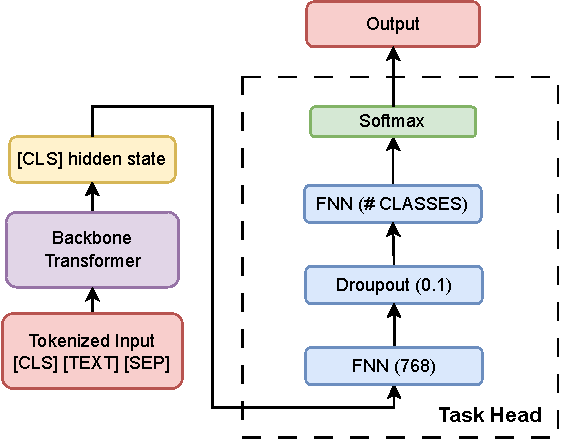
\includegraphics[width=0.7\linewidth]{img/transformer/fine_tune.pdf}
    \caption{Fine-tuning architecture for the classification task.}
    \label{fig:class-tune}
\end{figure}

We have used the following hyperparameters:
\begin{enumerate}
    \item Effective Batch size
    \footnote{By effective batch size we mean 
    $\text{gradient accumulation steps} \times \text{number of devices}
    \times \text{batch size}$
    }: 48
    \item Number of epochs: 2
    \item Sequence length: maximum 512 tokens with dynamic padding per batch
    \item Weight decay: 0
    \item Optimizer: AdamW with epsilon 1e-8, beta1 0.9, beta2 0.999.
    \item Scheduler: Linear warmup with 0.1 warmup ratio
    \item Unfrozen layers: 12
    \item Truncation: First 512 tokens
    \item Unfrozen Embeddings: False
\end{enumerate}
To find the learning rate (lr), we run a grid search for each model and task.
However, we quickly found out that the Fernet-News was more sensitive to the high lr and thus we couldn't apply the same lrs for both models.
For RobeCzech, we have used the following lrs:
\begin{enumerate}
    \item RobeCzech: $3e-5, 4.5e-5, 7.5e-5$
    \item Fernet-News: $1e-5, 2e-5, 3e-5$
\end{enumerate}

Grid search only run for 0.4 portion of the first epoch and lr with the best validation f1-macro score was selected.
For implementation, we have used \textit{Pytorch Lightning 2.0}, \textit{Huggingface Transformers 4.24} and \textit{Pytorch 2.0.0}.
The training was done on Ufal AIC cluster\footnote{https://aic.ufal.mff.cuni.cz/} on a single GeForce RTX 2080 Ti.

\subsection{GPT-3}
\label{sec:gpt-3}
We have chosen Ada version of GPT-3 as it is the cheapest.
Ada costs $0.00004\$/1k$ tokens for finetuning and $0.00016\$/1k$ tokens for a generation.
As the model architecture is not modifiable, the finetuning works
as text generation fine-tuning.
Thus we only provide query: Text of article and text completion: Class.
To save the cost we fine-tuned in a multi-task setting.
Thus for every task, we created a label in the format: \textit{Full\ Server Name} \textit{Category} \textit{Gender} \textit{Day of week}.

Example of the label:
\begin{quotation}
    \textit{Idnes.cz Sport Muž Pondělí}
\end{quotation}

The Ada model takes a maximum of 2048 tokens, we thus truncated documents to 1400 characters.
To save the costs we used Train-small (see \autoref{enum:train-small}) for finetuning and
Test-small (see \autoref{enum:test-small}) for inference.
We then finetuned for 2 epochs.
For comparison, we also additionally fine-tuned and evaluated the above models on the same dataset.

\section{Fine-tuning}
\label{sec:finetuning}
We were interested in ways to improve the performance of finetuning without changing the backbone model.
We tried 3 approaches mainly inspired by \cite{howardUniversalLanguageModel2018a} and \cite{sunHowFineTuneBERT2020}.
Note that \textbf{ULMFiT} is RNN architecture and thus its findings might not apply to transformers.
All the experiments were done on \textbf{RobeCzech} model, with settings as in \autoref{sec:robe-czech}
unless stated otherwise.

\subsection{Truncation}
\label{sec:truncation}
The base models are trained with truncation of the first 512 tokens as it was shown
the most effective by \cite{sunHowFineTuneBERT2020}. Due to the nature of the task,
we hypothesized that the last part might contain more relevant information:
\begin{quotation}
    Pro Idnes.cz Jana Křížová
\end{quotation}
We thus tried to truncate the text by taking the last
512 tokens.

\subsection{Task modeling}
\label{sec:task-modeling}
Both \cite{howardUniversalLanguageModel2018a} and \cite{sunHowFineTuneBERT2020}
found that further LM modeling on task dataset can improve performance.
We thus tried to use the same approach on our dataset.

For training LM we have used the following hyperparameters:
\begin{enumerate}
    \item Effective Batch size: 198
    \item Number of epochs: 10
    \item Sequence length: 512 tokens
    \item Sequence sampling: Cross document
    \item Masking: 15\% token change (80\% random, 10\% replace, 10\% keep)
    \item Optimizer: AdamW with epsilon 1e-8, beta1 0.9, beta2 0.98
    \item Unfrozen Embeddings: True
\end{enumerate}




\subsection{Gradual unfreezing with discriminative learning rates}
\label{sec:gradual-unfreezing}
This idea was inspired by \cite{howardUniversalLanguageModel2018a}.
When doing the gradual unfreezing, we unfreeze the layers in groups until all the layers are unfrozen.
The discriminative learning rate is a technique where the learning rate is different for each layer.
We set the discriminative factor to $0.95$ as in \cite{sunHowFineTuneBERT2020}.
The gradual unfreezing is not well described in ULMFiT, thus we tried two approaches:
\begin{enumerate}
    \item \textbf{GradDLR-12} Unfreeze 1 layer per epoch, starting from the last layer, and run for 12 epochs.
    \item \textbf{GradDLR-24} Unfreeze 1 layer per epoch,
    starting from the last layer, and run for 24 epochs(12 epochs in the full unfrozen state).
\end{enumerate}
The epoch lengths are adjusted, so that the total number of optimizer steps stays the same (full 2 epochs).

For both approaches, we unfreeze the classifier layer at epoch 0 with lr decaying from $1e-3$ to $ 5e-5$.
The first unfrozen layer has lr peak at best lr found at \autoref{sec:robe-czech} for given task.
The remaining layers are adjusted based on the discriminative learning rate.
Each unfrozen layer has its scheduler with the same setting as base model tuning (\autoref{sec:backbone}).
 However, it start scheduling when the layer was unfrozen.
The reaming setting stays the same as in base model tuning (\autoref{sec:backbone}).

\section{Final Model}
\label{sec:final-model}
Finally, we created a model that combines the best back-bone and the best finetuning approach.
